\addchap{Anhang}

\chapter{Zeitpläne}
\newpage
\section{Zeitplan 5. Semester}
\begin{figure}[H]
	\centering
	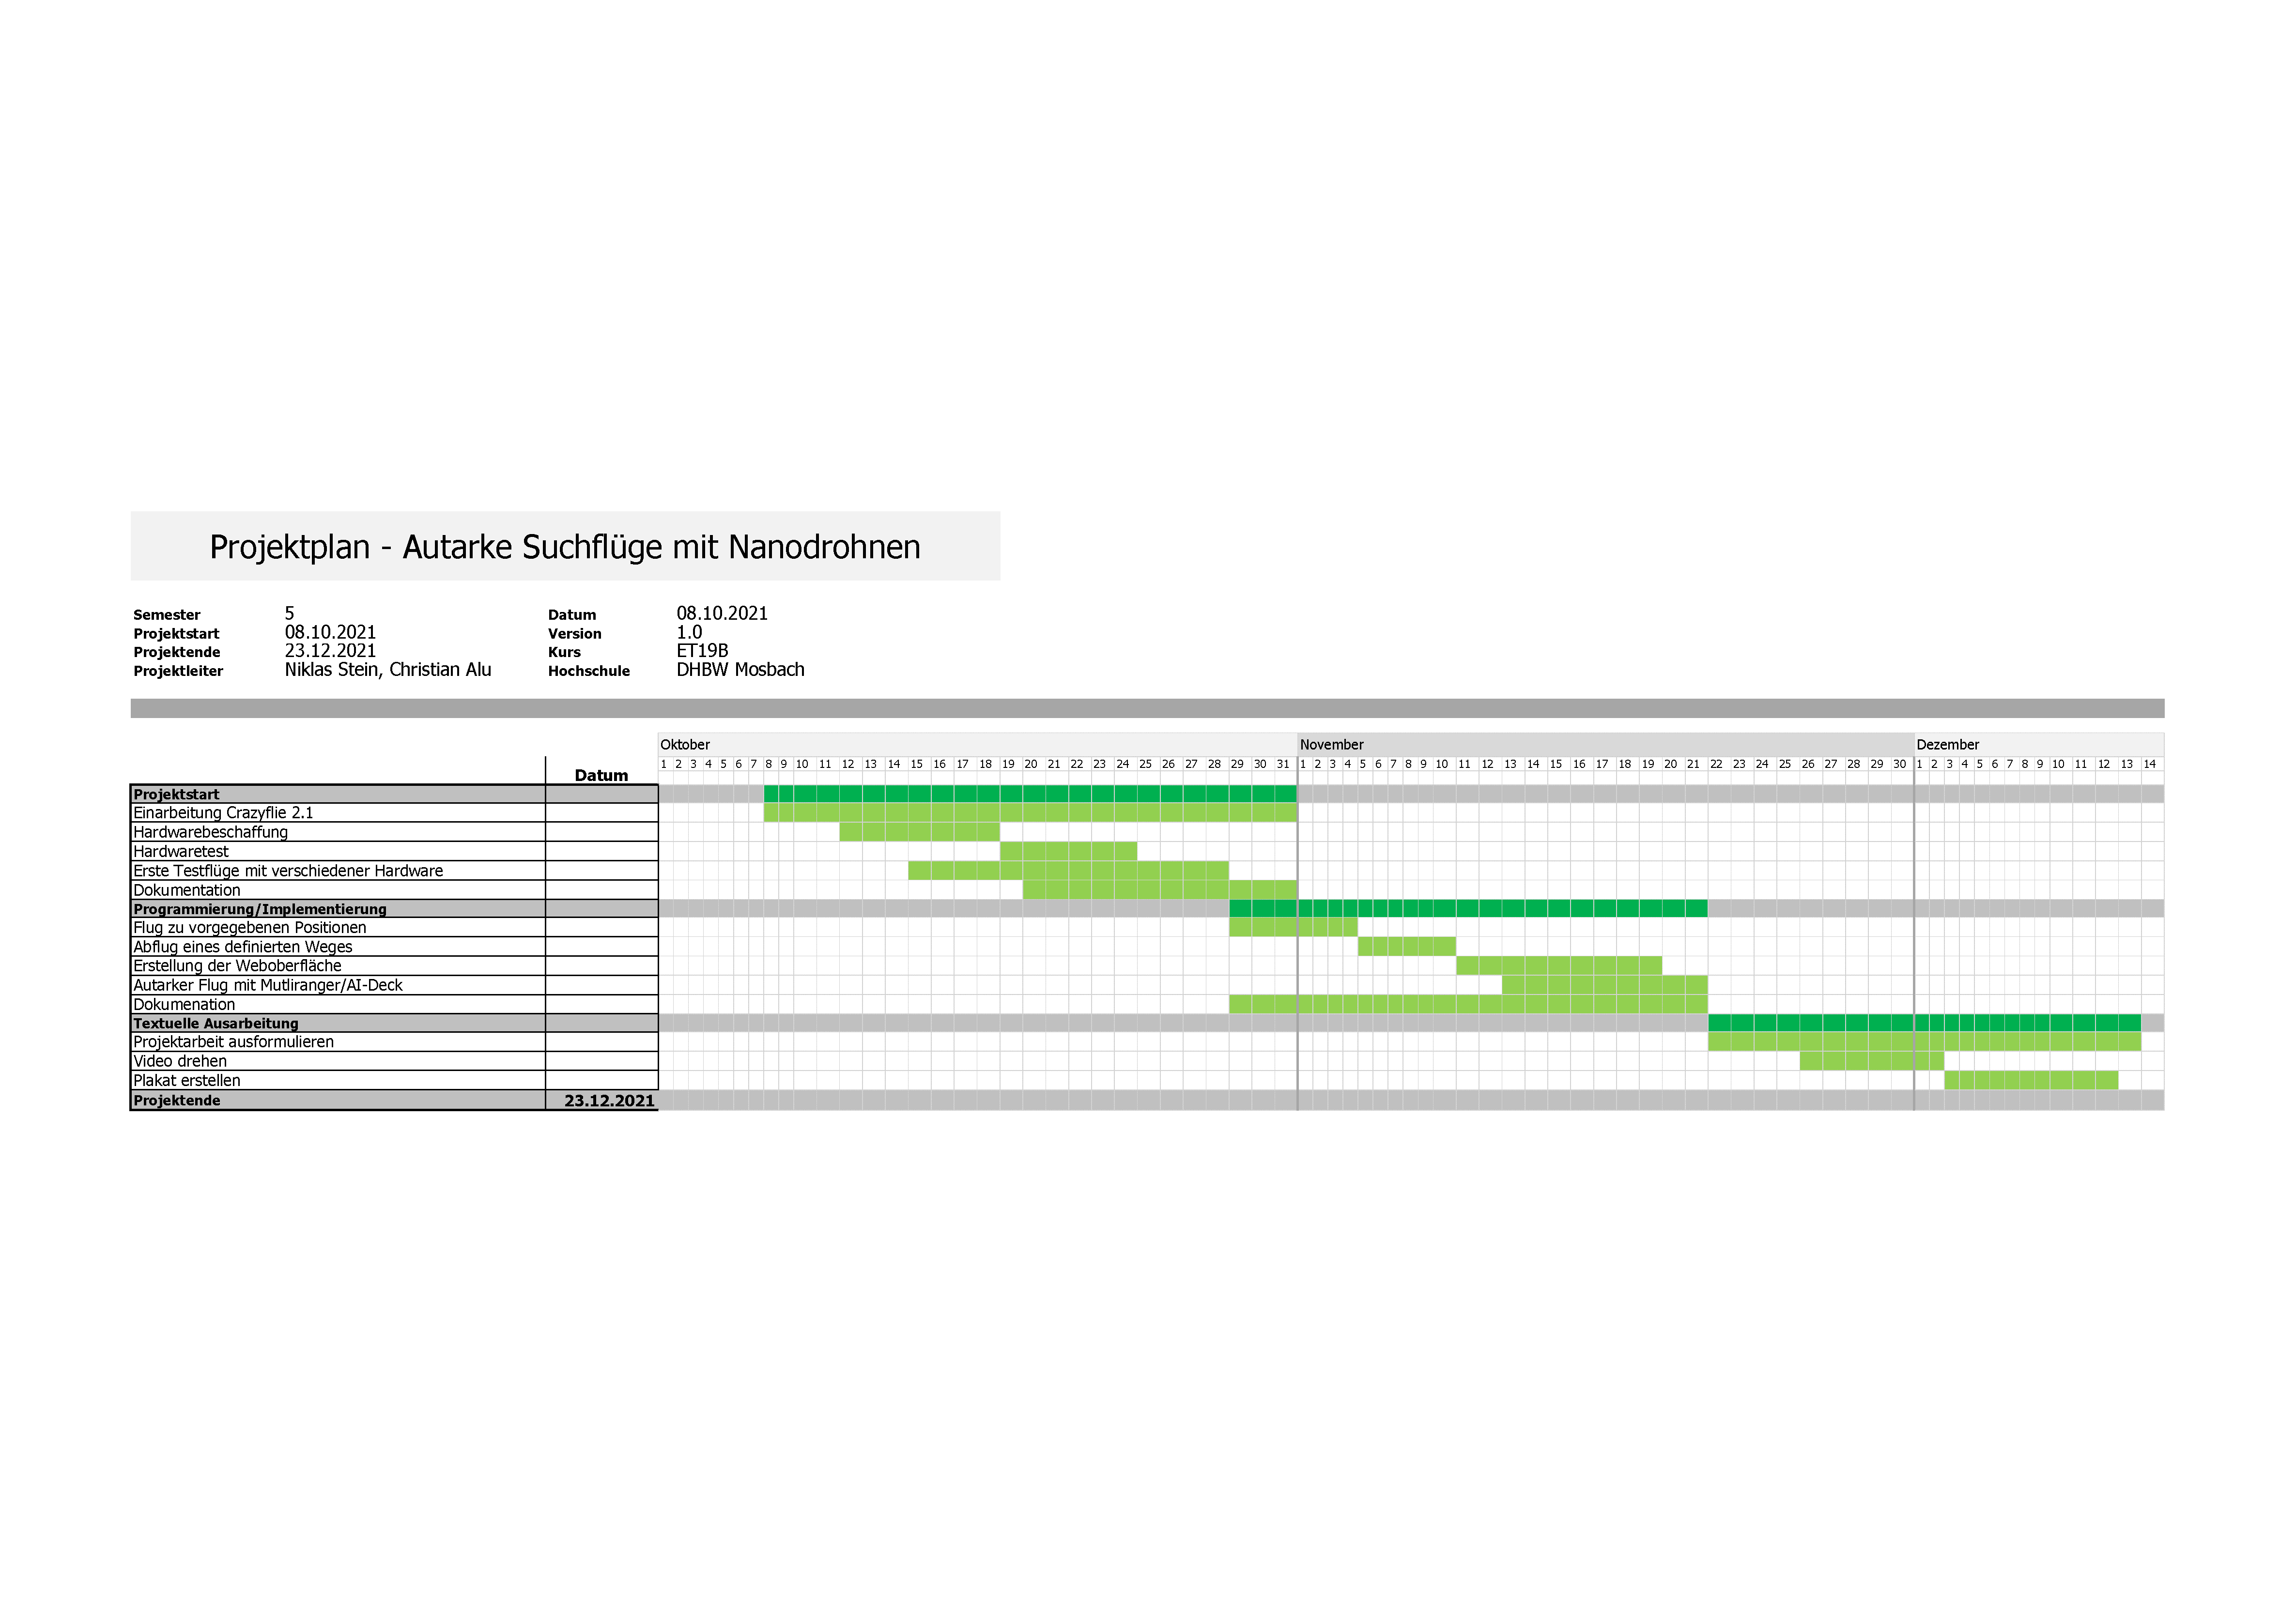
\includegraphics[angle=90, page=1,width=0.85\textwidth]{anhang/Projektplan.pdf}
	\caption{Zeitplan der Projektarbeit im 5. Semester  \protect \\ Quelle: Eigene Darstellung}
	\label{lab:Projektplan}
\end{figure}



\chapter{Datenblätter}
\newpage
	\section{Crazyflie 2.1}
	\begin{figure}[H]
	\centering
	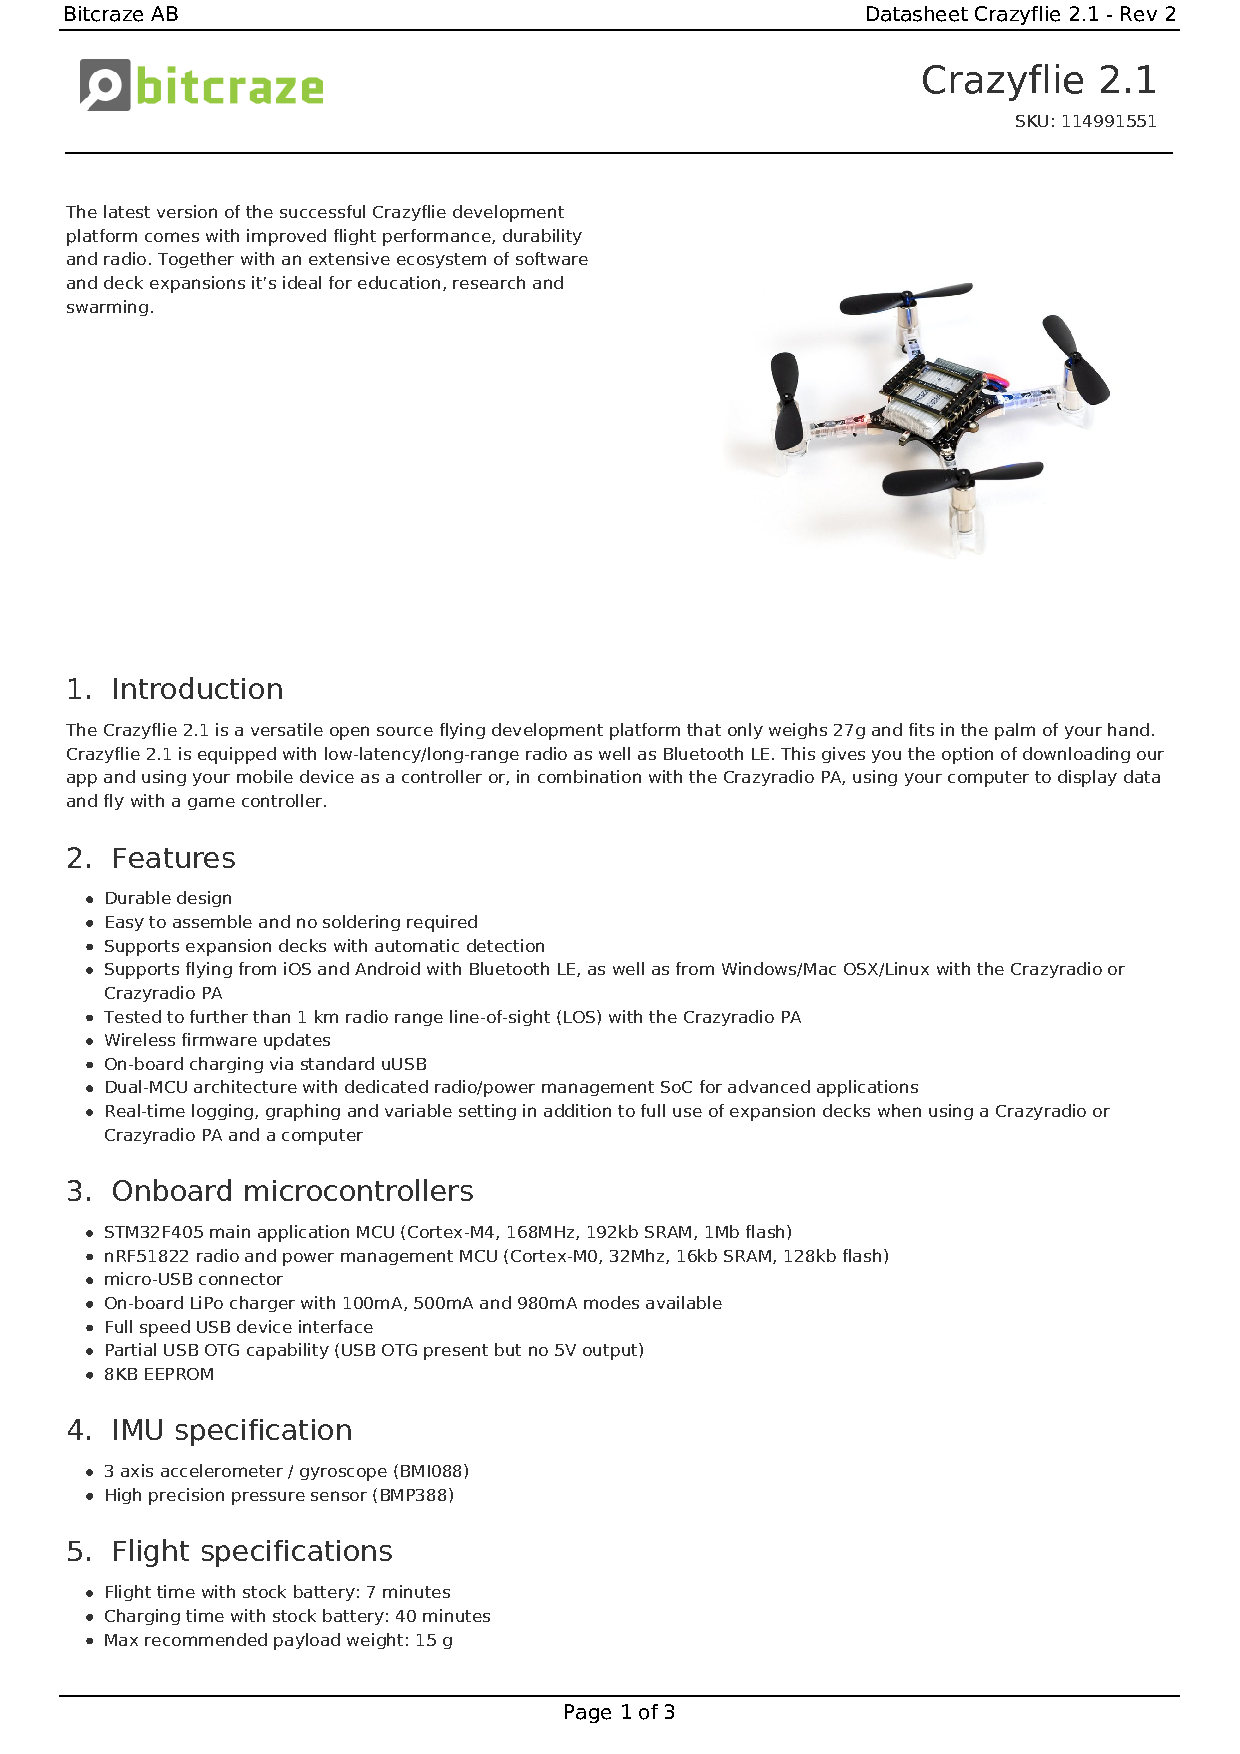
\includegraphics[page=1,width=.8\textwidth]{anhang/crazyfliedatasheet.pdf}
\end{figure}

	\begin{figure}[H]
	\centering
	\includegraphics[page=2,width=.8\textwidth]{anhang/crazyfliedatasheet.pdf}
\end{figure}

	\begin{figure}[H]
		\centering
		\includegraphics[page=3,width=.8\textwidth]{anhang/crazyfliedatasheet.pdf}
		\caption{Datenblatt Crazyflie 2.1 \protect \\ Quelle: \cite{.} }
		\label{lab:crazyfliedatasheet.pdf}
	\end{figure}

